\item \points{2d} {\bf Other feature maps}

You may have observed that it requires a relatively high degree $k$ to fit the given training data, and this is because the dataset cannot be explained (i.e., approximated) very well by low-degree polynomials. By visualizing the data, you may have realized that $y$ can be approximated well by a sine wave. In fact, we generated the data by sampling from $y = \sin(x) + \xi$, where $\xi$ is noise with Gaussian distribution. Please update the feature map $\phi$ to include a sine transformation as follows:

\begin{align}
\phi(x) = \left[\begin{array}{c} \sin(x) \\ 1 \\ x \\ x^2\\ \vdots \\x^k\end{array}\right]\in \mathbb{R}^{k+2} \label{eqn:feature-sine}
\end{align}

Complete the function |create_sin()| in |src/submission.py| to implement the updated feature map.  Again, ensure your code  works with a general $k$.  We will use $k=1,2,3,5,10,20$ as test cases. To verify a correct implementation, autograder test case |2d-7-basic| will create a plot in |src/large-sine.png|. Note that test |2d-7-basic| will NOT be awarded points and is used to test if your implementation can generate a plot similar to the following:

\begin{figure}[H]
  \centering
  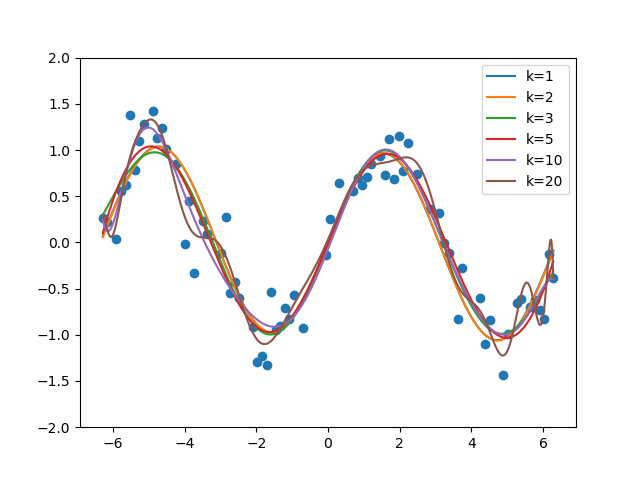
\includegraphics[width=0.65\linewidth]{02-featuremaps/large-sine.png}
  \centering
\caption{Polynomial regression with other features with kernel sizes 1,2,3,5,10 and 20. Visual impaired students can access the corresponding desmos plot \href{https://www.desmos.com/calculator/ikkytcrqyp}{here}}
\end{figure}
